%
% File coling2020.tex
%
% Contact: feiliu@cs.ucf.edu & liang.huang.sh@gmail.com
%% Based on the style files for COLING-2018, which were, in turn,
%% Based on the style files for COLING-2016, which were, in turn,
%% Based on the style files for COLING-2014, which were, in turn,
%% Based on the style files for ACL-2014, which were, in turn,
%% Based on the style files for ACL-2013, which were, in turn,
%% Based on the style files for ACL-2012, which were, in turn,
%% based on the style files for ACL-2011, which were, in turn, 
%% based on the style files for ACL-2010, which were, in turn, 
%% based on the style files for ACL-IJCNLP-2009, which were, in turn,
%% based on the style files for EACL-2009 and IJCNLP-2008...

%% Based on the style files for EACL 2006 by 
%%e.agirre@ehu.es or Sergi.Balari@uab.es
%% and that of ACL 08 by Joakim Nivre and Noah Smith

\documentclass[11pt]{article}
\usepackage{coling2020}
\usepackage{times}
\usepackage{url}
\usepackage{latexsym}
\usepackage{indentfirst}

\usepackage{times}
\usepackage{latexsym}
\usepackage{times}
\usepackage{soul}
\usepackage{url}
\usepackage{amsmath}
\usepackage{amsthm}
\usepackage{booktabs}
\usepackage{algorithm}
\usepackage{algorithmic}
\usepackage{amssymb}
\usepackage{longtable}
\usepackage{graphicx}
\usepackage{CJK}
\usepackage{multirow}
\usepackage{color}

%\setlength\titlebox{5cm}
\colingfinalcopy % Uncomment this line for the final submission

% You can expand the titlebox if you need extra space
% to show all the authors. Please do not make the titlebox
% smaller than 5cm (the original size); we will check this
% in the camera-ready version and ask you to change it back.


\title{论文提纲}

\author{屈原斌 \\
  首都师范大学 \\
    {\tt ybqu@cnu.edu.cn}}

\date{}

\begin{document}
\begin{CJK}{UTF8}{gkai}

\maketitle
\CJKindent
%\begin{abstract}

%\end{abstract}

% \section{今日进度}


\begin{itemize}
  \item [1.] 题目:A Comparison of Unsupervised Neural Encoders for Off-Topic Essay Detection
  \item [2.] 主要贡献:
  \begin{itemize}
    \item 使用神经网络学习编码器的获取主题特征
    \item 结合传统特征与神经网络特征进行离题分类检测
  \end{itemize}
  \item [3.] 实验结果:
  \begin{itemize}
    \item 实验数据:
    \begin{itemize}
      \item ICLE英文数据集:13个主题,共830篇作文
      \item 各档分数分布见表1:使用2.0-2.5分段作为离题作文,3.0-4.0分段作为切题作文,离题:切题=157:673(1:4.3)
    \end{itemize}
    \item 实验方案:
    \begin{itemize}
      \item 方案一:基于题目排序方案,见图1
      \item 方案二:基于相似度方案,见图2
      \item 方案三:使用baseline特征做SRC
    \end{itemize}
    \item 实验结果:见表2、3、4
  \end{itemize}
\end{itemize}

% Table generated by Excel2LaTeX from sheet '英文数据集'
\begin{table}[htbp]
  \centering
  \begin{tabular}{cccccccc}
    \hline
    \textbf{score} & \textbf{1} & \textbf{1.5} & \textbf{2} & \textbf{2.5} & \textbf{3} & \textbf{3.5} & \textbf{4} \\
    \hline
    \textbf{作文数} & 0     & 0     & 8     & 44    & 105   & 230   & 443 \\
    \hline
  \end{tabular}%
  \caption{ICLE各档分数分布}
  \label{tab:addlabel}%
\end{table}%


\begin{figure*}[htbp]\small
  \centering
  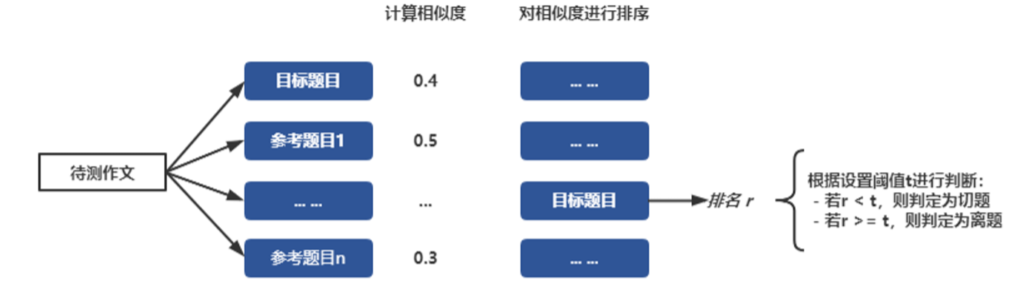
\includegraphics[width=0.8\linewidth]{fangan01.png}
  \caption{方案一:基于题目排序方案}
  \label{framework}
\end{figure*}

\begin{figure*}[htbp]\small
  \centering
  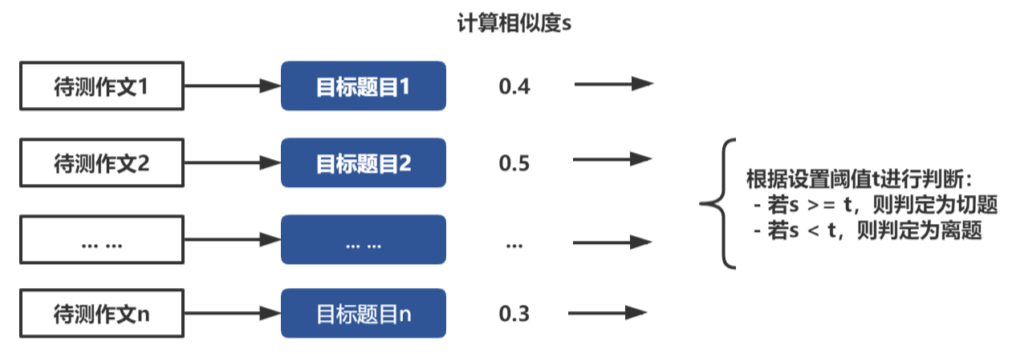
\includegraphics[width=0.8\linewidth]{fangan02.png}
  \caption{方案二:基于相似度方案}
  \label{framework}
\end{figure*}
% \section{工作详述}

% Table generated by Excel2LaTeX from sheet '3.0划分(Accuracy)'
\begin{table}[htbp]\small
  \centering
    \begin{tabular}{c|ccccccccc}
    \hline
    \multicolumn{3}{c}{\multirow{2}[0]{*}{\textcolor[rgb]{ 1,  0,  0}{}}} & \multirow{2}[0]{*}{\textbf{Accuracy}} & \multicolumn{3}{c}{\textbf{离题}} & \multicolumn{3}{c}{\textbf{不离题}} \\
    \multicolumn{3}{c}{} &       & \textbf{precision} & \textbf{recall} & \textbf{f1-score} & \textbf{precision} & \textbf{recall} & \textbf{f1-score} \\
    \hline
    \multicolumn{2}{c}{\multirow{2}[0]{*}{doc2vec}} & 开发集   & 0.9386  & 0.2000  & 0.0182  & 0.0333  & 0.9385  & 1.0000  & 0.9682  \\
    \multicolumn{2}{c}{} & 验证集   & 0.9334  & 0.3452  & 0.0192  & 0.0352  & 0.9382  & 0.9945  & 0.9655  \\
    \hline
    \multirow{6}[0]{*}{分类模型HT} & \multirow{2}[0]{*}{habilstm} & 开发集   & 0.9422  & 0.7000  & 0.1060  & 0.1794  & 0.9440  & 0.9974  & 0.9699  \\
    &       & 验证集   & 0.9364  & 0.5558  & 0.0920  & 0.1525  & 0.9424  & 0.9929  & 0.9670  \\
    \cline{2-10}
    & \multirow{2}[0]{*}{bert} & 开发集   & 0.9446  & 0.7200  & 0.1421  & 0.2299  & 0.9463  & 0.9974  & 0.9711  \\
    &       & 验证集   & 0.9301  & 0.4914  & 0.0870  & 0.1282  & 0.9418  & 0.9865  & 0.9636  \\
    \cline{2-10}
    & \multirow{2}[0]{*}{bert\_whitening} & 开发集   & 0.8602  & 0.0375  & 0.0321  & 0.0333  & 0.9345  & 0.9154  & 0.9246  \\
    &       & 验证集   & 0.8602  & 0.0297  & 0.0381  & 0.0333  & 0.9344  & 0.9152  & 0.9247  \\
    \hline
    \multirow{6}[0]{*}{生成模型HT} & \multirow{2}[0]{*}{lstm} & 开发集   & 0.9373  & 0.0000  & 0.0000  & 0.0000  & 0.9373  & 1.0000  & 0.9676  \\
    &       & 验证集   & 0.9322  & 0.0468  & 0.0094  & 0.0157  & 0.9375  & 0.9939  & 0.9649  \\
    \cline{2-10}
    & \multirow{2}[0]{*}{bert} & 开发集   & 0.9458  & 0.6267  & 0.1757  & 0.2721  & 0.9485  & 0.9961  & 0.9717  \\
    &       & 验证集   & 0.9386  & 0.6437  & 0.1493  & 0.2307  & 0.9458  & 0.9913  & 0.9680  \\
    \cline{2-10}
    & \multirow{2}[0]{*}{bert\_whitening} & 开发集   & 0.9084  & 0.1472  & 0.0571  & 0.0718  & 0.9388  & 0.9653  & 0.9518  \\
    &       & 验证集   & 0.9084  & 0.1005  & 0.0578  & 0.0732  & 0.9388  & 0.9653  & 0.9518  \\
    \hline
    \end{tabular}%
    \caption{方案一实验结果}
  \label{tab:addlabel}%
\end{table}%

% Table generated by Excel2LaTeX from sheet '3.0划分(Accuracy)'
\begin{table}[htbp]\small
  \centering
    \begin{tabular}{c|ccccccccc}
      \hline
      \multicolumn{3}{c}{\multirow{2}[1]{*}{}} & \multirow{2}[1]{*}{\textbf{Accuracy}} & \multicolumn{3}{c}{\textbf{离题}} & \multicolumn{3}{c}{\textbf{不离题}} \\
      \multicolumn{3}{c}{}  &       & \textbf{precision} & \textbf{recall} & \textbf{f1-score} & \textbf{precision} & \textbf{recall} & \multicolumn{1}{c}{\textbf{f1-score}} \\
      \hline
      \multicolumn{2}{c}{\multirow{2}[0]{*}{doc2vec}} & 开发集   & 0.9446  & 0.6000  & 0.0964  & 0.1582  & 0.9442  & 1.0000  & 0.9713  \\
      \multicolumn{2}{c}{} & 验证集   & 0.9373  & 0.3000  & 0.0253  & 0.0455  & 0.9387  & 0.9984  & 0.9676  \\
      \hline
      \multirow{6}[0]{*}{分类模型HT} & \multirow{2}[0]{*}{habilstm} & 开发集   & 0.9410  & 0.7000  & 0.1060  & 0.1794  & 0.9439  & 0.9961  & 0.9693  \\
      &       & 验证集   & 0.9377  & 0.5133  & 0.0770  & 0.1334  & 0.9416  & 0.9952  & 0.9677  \\
      \cline{2-10}
      & \multirow{2}[0]{*}{bert} & 开发集   & 0.9422  & 0.6167  & 0.1199  & 0.1963  & 0.9451  & 0.9961  & 0.9699  \\
      &       & 验证集   & 0.9337  & 0.5328  & 0.0775  & 0.1202  & 0.9414  & 0.9910  & 0.9655  \\
      \cline{2-10}
      & \multirow{2}[0]{*}{bert\_whitening} & 开发集   & 0.1289  & 0.0639  & 0.9262  & 0.1192  & 0.9470  & 0.0747  & 0.1381  \\
      &       & 验证集   & 0.1289  & 0.0637  & 0.9416  & 0.1194  & 0.9504  & 0.0746  & 0.1383  \\
      \hline
      \multirow{6}[0]{*}{生成模型HT} & \multirow{2}[0]{*}{lstm} & 开发集   & 0.9373  & 0.0000  & 0.0000  & 0.0000  & 0.9373  & 1.0000  & 0.9676  \\
      &       & 验证集   & 0.9373  & 0.0000  & 0.0000  & 0.0000  & 0.9373  & 1.0000  & 0.9677  \\
      \cline{2-10}
      & \multirow{2}[0]{*}{bert} & 开发集   & 0.9373  & 0.0000  & 0.0000  & 0.0000  & 0.9373  & 1.0000  & 0.9676  \\
      &       & 验证集   & 0.9373  & 0.0000  & 0.0000  & 0.0000  & 0.9373  & 1.0000  & 0.9677  \\
      \cline{2-10}
      & \multirow{2}[0]{*}{bert\_whitening} & 开发集   & 0.1651  & 0.0629  & 0.8823  & 0.1171  & 0.9361  & 0.1171  & 0.2078  \\
      &       & 验证集   & 0.1651  & 0.0628  & 0.8845  & 0.1172  & 0.9380  & 0.1170  & 0.2080  \\
      \hline
    \end{tabular}%
  \caption{方案二实验结果}
  \label{tab:addlabel}%
\end{table}%

% Table generated by Excel2LaTeX from sheet '3.0划分(Accuracy)'
\begin{table}[htbp]\small
  \centering
  \begin{tabular}{cccccccc}
    \hline
    \multirow{2}[0]{*}{} &       & \multicolumn{3}{c}{离题(score=2.0-3.5)} & \multicolumn{3}{c}{切题(score=4.0)} \\
    & Accuracy & Precision & Recall & F1-score & Precision & Recall & F1-score \\
    \hline
    c-SVC & 0.9349  & 0.0000  & 0.0000  & 0.0000  & 0.9372  & 0.9975  & 0.9663  \\
    \hline
    nu-SVC & 0.9325  & 0.2000  & 0.0154  & 0.0286  & 0.9381  & 0.9936  & 0.9650  \\
    \hline
  \end{tabular}%
  \caption{方案三实验结果}
  \label{tab:addlabel}%
\end{table}%


\end{CJK}
\end{document}

% include your own bib file like this:


%\begin{thebibliography}{}

%\bibitem[\protect\citename{Aho and Ullman}1972]{Aho:72}
%Alfred~V. Aho and Jeffrey~D. Ullman.
%\newblock 1972.
%\newblock {\em The Theory of Parsing, Translation and Compiling}, volume~1.
%\newblock Prentice-{Hall}, Englewood Cliffs, NJ.

%\bibitem[\protect\citename{{American Psychological Association}}1983]{APA:83}
%{American Psychological Association}.
%\newblock 1983.
%\newblock {\em Publications Manual}.
%\newblock American Psychological Association, Washington, DC.

%\bibitem[\protect\citename{{Association for Computing Machinery}}1983]{ACM:83}
%{Association for Computing Machinery}.
%\newblock 1983.
%\newblock {\em Computing Reviews}, 24(11):503--512.

%\bibitem[\protect\citename{Chandra \bgroup et al.\egroup }1981]{Chandra:81}
%Ashok~K. Chandra, Dexter~C. Kozen, and Larry~J. Stockmeyer.
%\newblock 1981.
%\newblock Alternation.
%\newblock {\em Journal of the Association for Computing Machinery},
%  28(1):114--133.

%\bibitem[\protect\citename{Gusfield}1997]{Gusfield:97}
%Dan Gusfield.
%\newblock 1997.
%\newblock {\em Algorithms on Strings, Trees and Sequences}.
%\newblock Cambridge University Press, Cambridge, UK.

%\bibitem[\protect\citename{Rasooli and Tetreault}2015]{rasooli-tetrault-2015}
%Mohammad~Sadegh Rasooli and Joel~R. Tetreault. 2015.
%\newblock {Yara parser: {A} fast and accurate dependency parser}.
%\newblock \emph{Computing Research Repository}, arXiv:1503.06733.
%\newblock Version 2.

%\bibitem[\protect\citename{Borschinger and Johnson}2011]{borsch2011}
%Benjamin Borschinger and Mark Johnson. 2011.
%\newblock A particle filter algorithm for {B}ayesian wordsegmentation.
%\newblock In \emph{Proceedings of the Australasian Language Technology Association %Workshop 2011}, pages 10--18, Canberra, Australia.

%\end{thebibliography}

